\icode{E-MD-SI-L2-261114-006}
如图所示，\(AO\)、\(AB\)、\(AC\) 是竖直平面内的三根固定的细杆，\(A\)、\(O\) 位于同一圆周上，\(A\) 点位于圆周的最高点，\(O\) 点位于圆周的最低点，每一根细杆上都套有一个光滑的小球（图中未画出），三个环都从 \(A\) 点无初速地释放，用 \(T_1\)、\(T_2\)、\(T_3\) 表示各环到 \(O\)、\(B\)、\(C\) 时所用的时间，则\paren[]
	
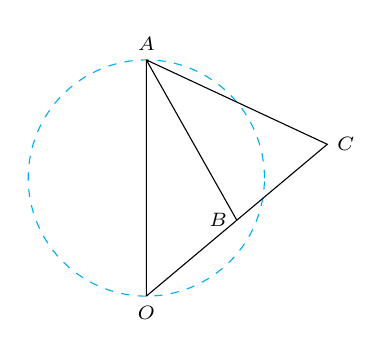
\begin{tikzpicture}[font=\scriptsize]
	\draw[dashed,cyan] (0,1.5) circle(1.5);
	\draw (0,0)node[below]{\(O\)}--(40:3)node[right]{\(C\)}--(0,3)node[above]{\(A\)} (40:1.5)node[left]{\(B\)}--(0,3) (0,0)--(0,3);
\end{tikzpicture}
\begin{choices}
	\item \(T_1 > T_2 > T_3\)
	\item \(T_3 < T_1 < T_2\)
	\item \(T_1 < T_2 < T_3\)
	\item \(T_3 > T_1 > T_2\)
\end{choices}
\begin{answer}
    D\qquad 提示：
\end{answer}